%%%%%%%%%%%%%%%%%%%%%%%%%%%% MPM %%%%%%%%%%%%%%%%%%%%%%%%%%%%
\section{Meyer-Peter \& Müller (1948)}
\label{app:MPM}

The most common formula, and still currently used nowadays, is the Meyer-Peter \& Müller \cite{MPM} formula also noted MPM. 
It was elaborated from bedload experiments in flumes for median grain sizes between 0.4 à 29 mm. 
Sediment transport is computed above a critical stress $\tau_c = 0.047$ and the solid transport rate is computed from :
\bequ
    Q_s = \frac{C_{MPM}}{1-n} B\sqrt{R g d_{50}^3} \left(\theta^*-\theta_c \right)^{\frac{3}{2}}
\eequ
where the adimensional efficient shear stress $\theta^*$ is defined as
\bequ
	\theta^* = \left(\frac{K}{K_p}\right)^{\frac{3}{2}} \theta
\eequ
\begin{itemize}
	\item $C_{MPM}$ is a coefficient for the MPM formula. In \courlis, $C_{MPM} = 8$ ;
	\item $n$ represents the sediment porosity, by default $n=0.25$. Its value can be changed by the user via the option \telkey{POROSITE};
	\item $d_{50}$ is the median grain diameter ;
	\item $R$ the relative reduced density $R=\frac{\rho_s}{\rho_w}-1$.
\end{itemize}

The Shields parameter $\theta$ is computed from 
\bequ
    \label{eq:shields}
    \theta = \frac{U^2}{RK^2R_h^{\frac{1}{3}}d_{50}} 
\eequ

\nomenclature{$C_{MPM} $}{Meyer-Peter \& Müller coefficient \nomunit{$\emptyset$}}
\nomenclature{$U$}{Average velocity across section \nomunit{$m.s^{-1}$}}
\nomenclature{$d_m$}{Mean diameter \nomunit{$m$}}
\nomenclature{$R$}{Relative reduced density \nomunit{$\emptyset$}}
\nomenclature{$\rho_s$}{Sediment density \nomunit{$kg.m^{-3}$}}
\nomenclature{$\rho_w$}{Water density \nomunit{$kg.m^{-3}$}}
\nomenclature{$Q_s$}{Solid discharge \nomunit{$m^3.s^{-1}$}}
\nomenclature{$B$}{Bed width \nomunit{$m$}}
\nomenclature{$d_{50}$}{Median diameter \nomunit{$m$}}
\nomenclature{$K_p$}{Skin friction coefficient \nomunit{$m^{\frac{1}{3}}.s^{-1}$}}
\nomenclature{$\theta$}{Shields number \nomunit{$\emptyset$}}
\nomenclature{$\tau$}{Shear stress \nomunit{$Pa$}}
\nomenclature{$u^*$}{Vitesse de frottement sur le fond \nomunit{$m.s^{-1}$}}
\nomenclature{$\tau_c$}{Critical shear stress \nomunit{$Pa$}}
\nomenclature{$\theta_c$}{Critical Shields number \nomunit{$\emptyset$}}
\nomenclature{$\theta^*$}{Adimensional efficient shear stress \nomunit{$\emptyset$}}
\nomenclature{$\tau^*$}{Efficient shear stress  \nomunit{$Pa$}}
\nomenclature{$\Phi^*$}{Einstein number \nomunit{$\emptyset$}}
\nomenclature{$n$}{Porosity \nomunit{$\emptyset$}}
\nomenclature{$\nu$}{Kinematic viscosity of water \nomunit{$Pa.s$}}
\nomenclature{$d_{16}$}{Diameter for which 16\% of grains are smaller (fine fraction) \nomunit{$m$}}
\nomenclature{$d_{84}$}{Diameter for which 84\% of grains are smaller (coarse fraction) \nomunit{$m$}}
\nomenclature{$d_{90}$}{Diameter for which 90\% of grains are smaller \nomunit{$m$}}

The MPM formula is not fit for sand transport nor high slopes problems. Moreover, it often underestimates gravel transport during periods of low flow \cite{lefort}.

%%%%%%%%%%%%%%%%%%%%%%%%%%%% LEFORT %%%%%%%%%%%%%%%%%%%%%%%%%%%%
\section{Lefort (2015)}
\label{app:lefort}

In Lefort \cite{lefort} equation, an adimensional diameter $d_m^*$ is defined such as:
\bequ
	d_m^* = d_m {\left[\frac{gR}{\nu^2}\right]}^{\frac{1}{3}}
\eequ
where $\nu$ is the water kinematic viscosity.

The transition discharge $Q_0$ which separates partiel bedload from general bedload is chosen such as :
\bequ
 	\frac{Q_0}{B\sqrt{g(Rd_{m})^3}} = C(d_m^*) \left(\frac{d_m}{B}\right)^{\frac{1}{3}} \left(\frac{K}{K_p}\right)^{-0.5} J^{-m_0}
\eequ
with $C(d_m^*)$ a function to describe the Shields stress variation with the mean grain diameter:
\bequ
	C(d_m^*) = 0.0444 \left[1+\frac{15}{1+d_m^*}-1.5\exp{\left(-\frac{d_m^*}{75}\right)}\right] 
\eequ
The shear stress increase with slope is done thanks to the exponent $m_0$ such as 
\bequ
	 m_0 = 1.6 +0.06 \log_{10}(J)
\eequ

The solid discharge is then estimated as :
\bequ
	Q_s = \frac{1.7}{1-n}\: Q \: J^m \frac{R+1}{R^{1.65}} \left[0.5\left(\frac{d_{84}}{d_{50}}\frac{d_{50}}{d_{16}}\right)\right]^{0.2} C_{dune} \frac{F(Q)}{(R+1)(1-n)}
\eequ
with $m = 1.8 +0.08\log_{10}(J)$

The term $0.5 \left(\frac{d_{84}}{d_{50}}\frac{d_{50}}{d_{16}}\right)$ relates to the particle size range.

The dune correction coefficient $C_{dune}$ serves to model the increase in friction due to the development and the transport of dunes. It is set for grain diameters above 0.6 mm. According to Lefort \cite{lefort}, it has little influence on the results. 
\bequ
	 C_{dune} = \left\{
        \begin{array}{ll}
            1-1.4\exp\left(-0.9 \left(\frac{K}{K_p}\right)^2\left(\frac{Q}{Q_0}\right)^{0.5}\right) \qquad \textrm{if}\quad d_m^*<14 \quad \textrm{and} \quad \frac{K}{K_p}<0.63, \\
            1 \qquad \textrm{otherwise}\\
        \end{array}
    \right.
\eequ

The discharge function $F$ describes the partial bedload of fine particles and general tranport, first bedload and then bedload and suspended load, via the following expression :
\bequ
	F(Q) = \left\{
        \begin{array}{ll}
            0.06 \: C_M \: \frac{Q}{Q_0} \qquad \textrm{if}\quad Q<Q_0, \\
            {\left[0.6{\left(1-0.938{\left(\frac{Q_0}{Q}\right)}^{0.284}\right)}^{1.66}\right]}^{m_z} \qquad \textrm{otherwise}\\
        \end{array}
    \right.
\eequ
with $m_z$ the add-on exponent for solid discharge during the transition between bedload and suspension:
\bequ
	m_z = \left\{
        \begin{array}{ll}
            1+\frac{0.38}{{d_m^*}^{0.45}} {\left(\frac{Q}{B\sqrt{gd_m^3}}\right)}^{0.192} \qquad \textrm{if}\quad Q>3.4Q_0, \\
            1 \qquad \textrm{otherwise}\\
        \end{array}
    \right.
\eequ
and $C_M$ a reduction factor of transport for partial bedload :

\bequ
	C_M = \left\{
        \begin{array}{ll}
            \frac{1}{200}\left(\frac{Q}{B\sqrt{gJd_{m}^3}}+2.5\right) \qquad \textrm{if}\quad \frac{Q}{B\sqrt{gJd_{m}^3}}<200, \\
            1 \qquad \textrm{otherwise}\\
        \end{array}
    \right.
\eequ

When the ratio $\frac{K}{K_p}$ is unknown, an alternative is suggested and can be activated in \courlis with the boolean \telkey{ROUGHNESS RATIO WITH QSTAR FOR LEFORT}.

When set to \telkey{TRUE}, the friction coefficient ratio is given by :
\bequ
	\frac{K}{K_p} = \left\{
        \begin{array}{ll}
            0.75 {\left(\frac{Q}{200B\sqrt{gJd_{84}^3}} \right)}^{0.23}  \qquad \textrm{if}\quad \frac{Q}{B\sqrt{gJd_{84}^3}}<200, \\
            0.75 \qquad \textrm{otherwise}\\
        \end{array}
    \right.
\eequ

%%%%%%%%%%%%%%%%%%%%%%%%%%%% RECKING 2013 %%%%%%%%%%%%%%%%%%%%%%%%%%%%
\section{Recking (2013)}
\label{app:recking2013}

The Recking \cite{recking2013} transport law is based on the surface diameter $d_{84}$ to characterize the bed friction and its ratio with the median diameter to characterize the particle size range. 

A mobility stress $\theta^*_m$ is defined, to separate partial bedload from general bedload. This parameter is also called the Recking number \cite{lefort}. 
This mobility stress is supposed constant for sands ($d_m < 2mm : \theta^*_m=0.045$) and is evaluated for other particles by :
\bequ
	\theta^*_m = \left(5J + 0.06\right){\left(\frac{d_{84}}{d_{50}}\right)}^{4.4\sqrt{J}-1.5}
\eequ
The associate Shields stress is computed by :
\bequ
	\theta_{84}^* = \frac{J}{Rd_{84} \left(\frac{2}{B}+74 p^{2.6}(gJ)^p \left(\frac{Q}{B}\right)^{-2p} d_{84}^{3p-1}\right)}
\eequ
with \[p = \left\{
        \begin{array}{ll}
            0.2275 \qquad \textrm{if}\quad \frac{Q}{B\sqrt{gJd_{84}^3}}<100, \\
            0.3025 \qquad \textrm{otherwise}\\
        \end{array}
    \right.\]
An Einstein number is then defined from this two stresses by :
\bequ
	 \Phi = \frac{14{\theta_{84}^{*}}^{2.5}}{1+{\left(\frac{\theta^*_m}{\theta_{84}^*}\right)}^4}
\eequ
Finally, the solid discharge can be written as :
\bequ
	Q_s = \frac{B}{1-n} \Phi \sqrt{gRd_{84}^3}
\eequ

%%%%%%%%%%%%%%%%%%%%%%%%%%%% RECKING 2015 %%%%%%%%%%%%%%%%%%%%%%%%%%%%
\section{Recking (2015)}
\label{app:recking2015}

In 2015, new estimations for the mobility stress were added to the Recking formula to discriminate riffle-pools and alternate bars (where it depends on $\frac{d_{84}}{d_{50}}$) from other morphologies (especially rivers with flat beds and narrow channels)\cite{recking2015}. Examples of those different morphologies are shown in Figure \ref{fig:morpho_recking2015}. 

For these latter, $\theta^*_m$ expression becomes :
\bequ
	\theta^*_m = 1.5 J^{0.75}
	\label{eq:recking2015_others}
\eequ
For sand bed rivers, this choice does not matter because the Shield number is generally high enough so errors generated by taking the average stress over the section remains negligeable. 

In \courlis, the expression of $\theta^*_m$ is set by the option \telkey{MORPHOLOGY OPTION RECKING 2015}. By default, it is equal to 1 for riffle-pools and alternate bars but it can be set to 2 to use the expression above (Equation \ref{eq:recking2015_others}).

The Shields number is computed by default from the discharge (\telkey{SHIELDS SHEAR STRESS WITH DISCHARGE FOR RECKING 2015 = TRUE}) :

\bequ
\theta_{84}^* = 0.015\frac{J}{R} {\left(\frac{Q}{B\sqrt{gJd_{84}^3}}\right)}^{2p} \frac{1}{p^{2.5}}
\eequ
with \[p = \left\{
        \begin{array}{ll}
            0.23 \qquad \textrm{if}\quad \frac{Q}{B\sqrt{gJd_{84}^3}}<100, \\
            0.31 \qquad \textrm{otherwise}\\
        \end{array}
    \right.\]
Otherwise, the Shields number is computed from the hydraulic radius :
\bequ
	\theta_{84}^* = \frac{JR_h}{Rd_{84}}
\eequ

\begin{figure}[htb!]
    \centering
    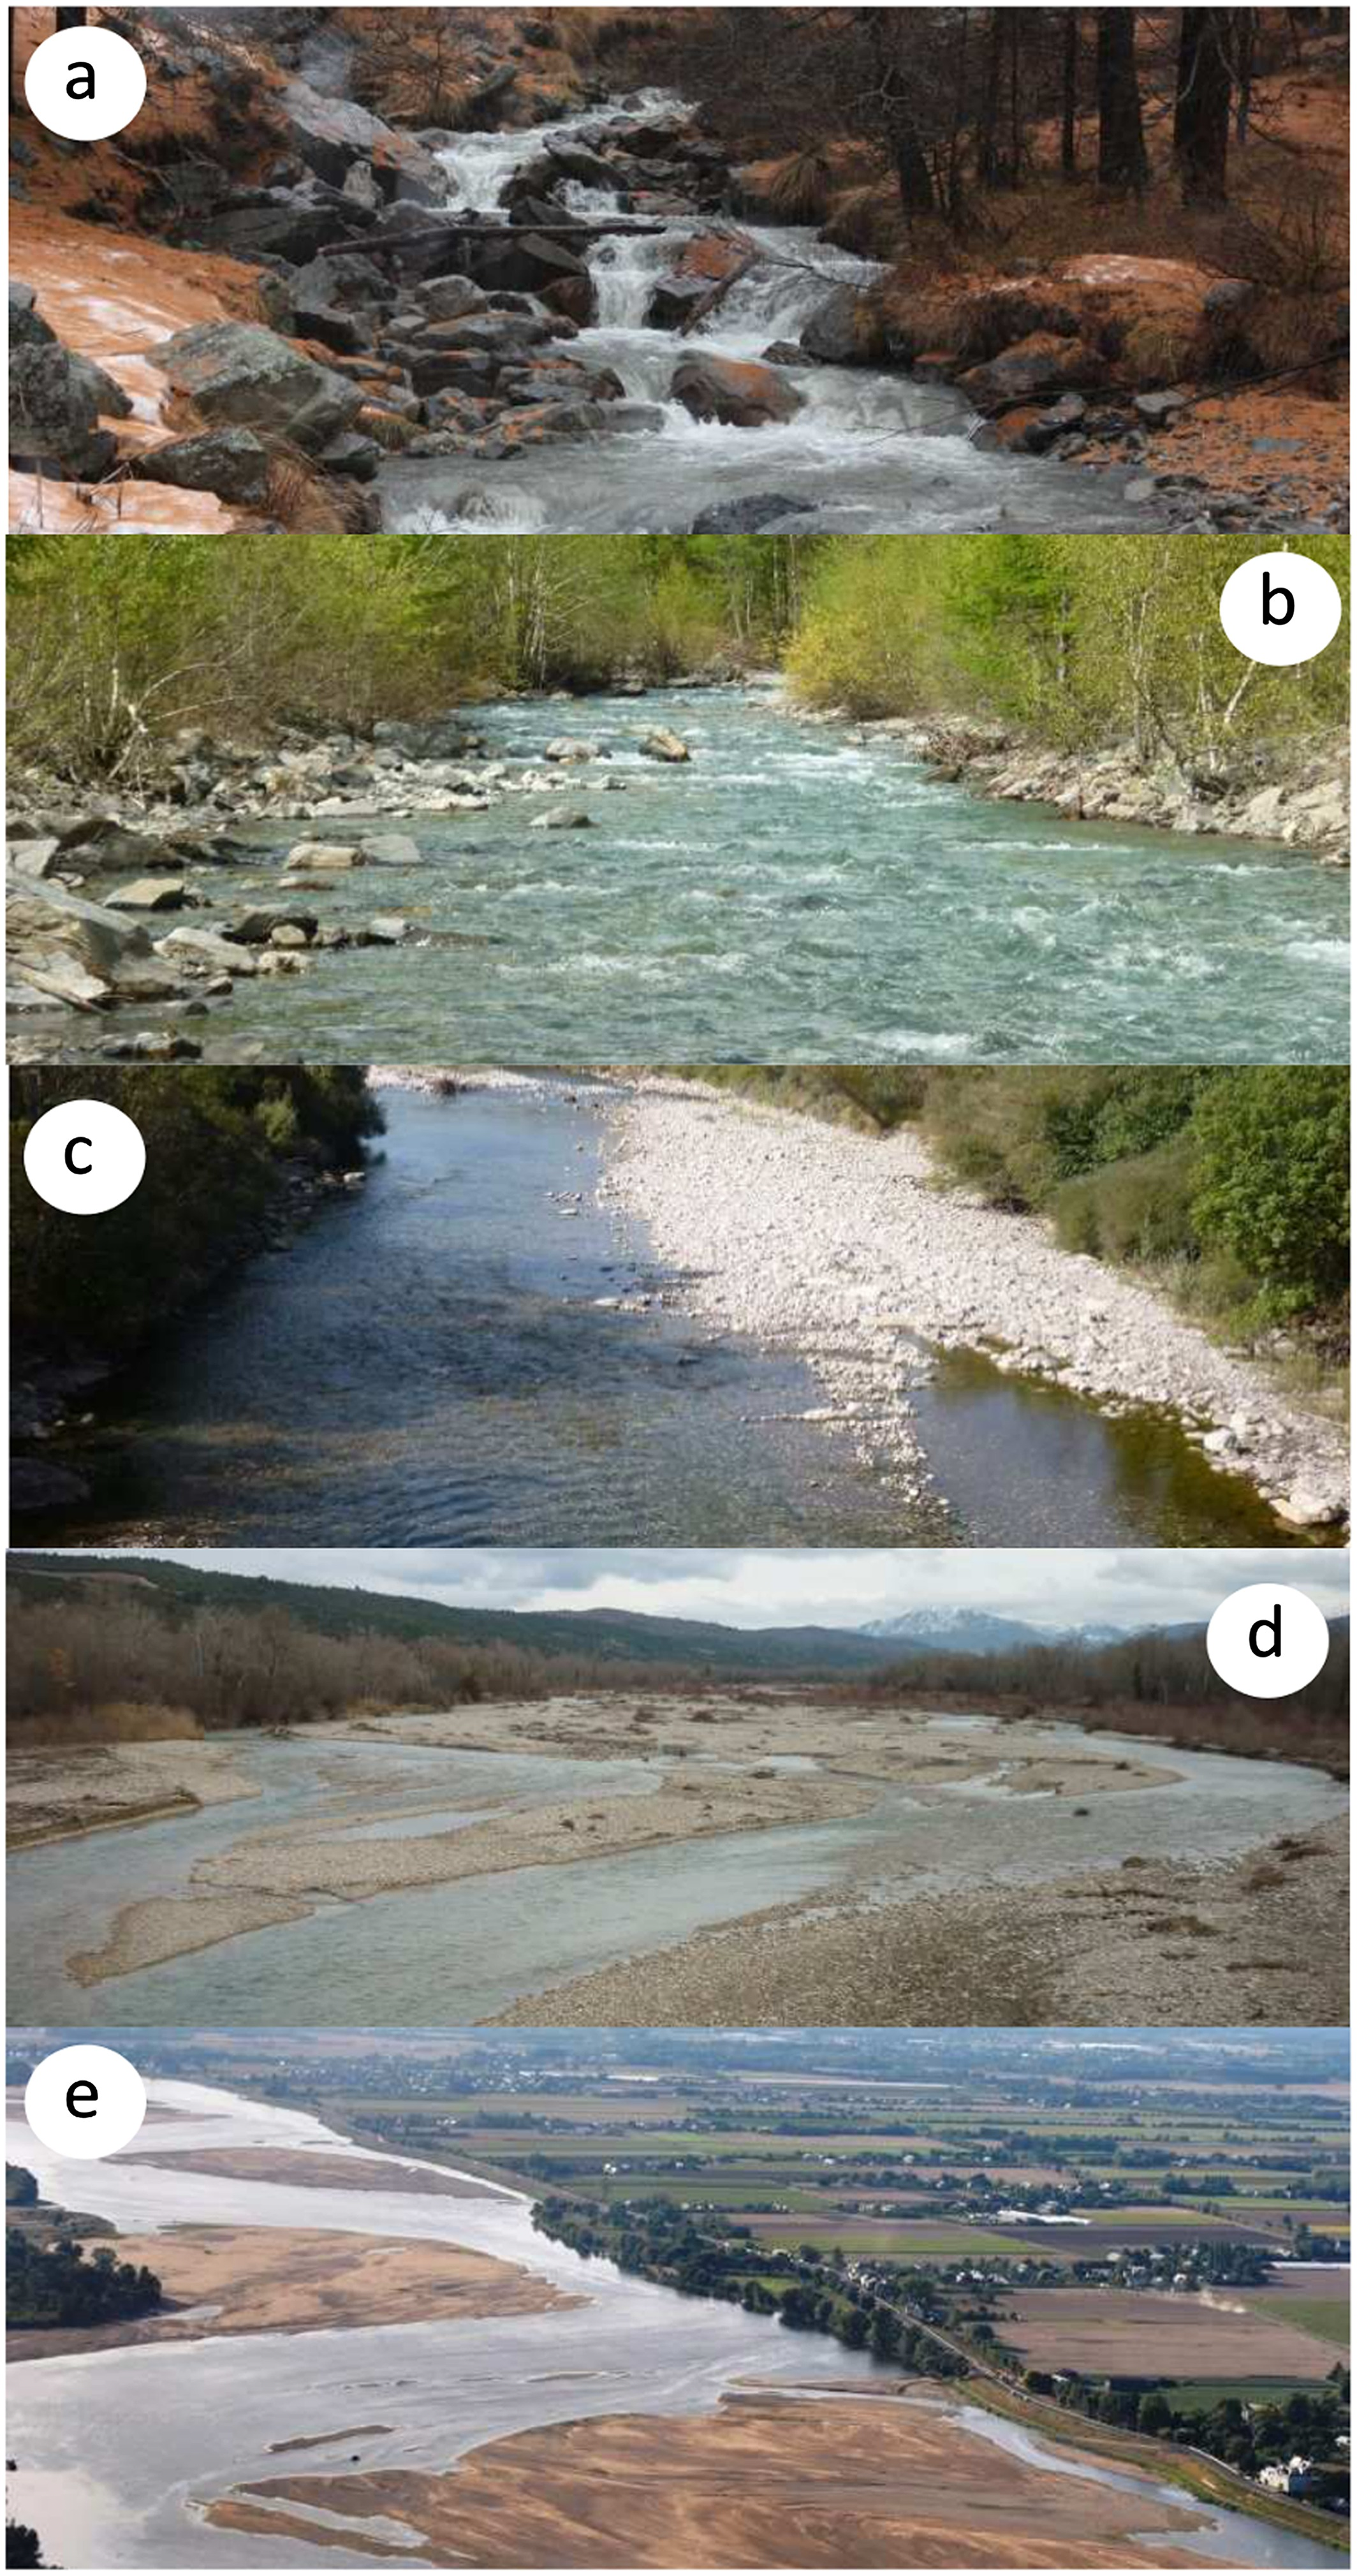
\includegraphics[width=0.45\textwidth]{./graphics/recking2015.jpg}
    \caption{(a) A step-pool stream (Tinée), (b) a plane-bed stream (Byasse), (c) a riffle-pool stream (Drac), (d) a braided stream (Bléone), (e) a sand-bed river (Loire). © S. Rodrigez. from Recking et al. \cite{recking2015}}
    \label{fig:morpho_recking2015}
\end{figure}
